\section{Intensive Experiments for Performance Insights}
\label{sec:intensive-experiments}

\subsection{Evaluation Platform Settings}
\subsubsection{Experimental Environment.}
\label{subsubsec:eval-exp-env}
\textcolor{blue}{
All experiments were conducted on two server-class Amazon Web Services (AWS) instances running Ubuntu 24.04.4 LTS. 
The \phantomsection\label{para:exp-setup-cpu}central processing unit (CPU)-based baselines were evaluated on an m7i.metal-24xl instance equipped with an Intel Xeon Platinum 8488C CPU with 48 physical cores, 96 hardware threads, 105 MB L3 cache, and 405 GB RAM.
In our experiments, CPU implementations use at most 48 software threads, assigning at most one worker thread to each physical core and avoiding multithreading.
The \phantomsection\label{para:exp-setup-gpu}graphics processing unit (GPU)-based baselines were evaluated on a g7e.8xlarge instance equipped with an NVIDIA RTX PRO 6000 Blackwell Server Edition GPU with 96 GB GPU memory, compute capability 12.0, NVIDIA driver 595.71.05, and CUDA 13.2.
We used two separate instances because the CPU baselines require a bare-metal instance to expose memory-system information, whereas AWS GPU instances do not provide this capability. 
All code was compiled with -O3 optimizations. The software stack included g++ 13.3.0, CMake 4.3.1, and CUDA Toolkit 13.2.
Parallel execution for our implementations follows their target architectures: X-Blossom-Pro (XB-Pro) relies on C++ \texttt{std::thread} backed by pthreads, while X-Blossom++ (XB++) launches CUDA kernels.
}

\subsubsection{Datasets.}
The ten real-world graph datasets used to evaluate our baselines are summarized in Table~\ref{tab:graph-metrics}.
% basic size
Drawn from the SNAP collection \cite{SNAP_Dataset}, these datasets span diverse application domains and exhibit substantial variation in the numbers of nodes and edges.
\phantomsection\label{para:real-world-sparse-datasets}
\textcolor{blue}{In this paper, we focus on real-world sparse graph datasets to align the evaluation with the graph structures commonly observed in large-scale network-analysis workloads.
% , where irregular degree distributions, sparse connectivity, and frontier-dependent parallelism strongly affect CPU and GPU behavior.
}
% other properties
In addition to the number of nodes and edges, we report several structural properties to better characterize each graph, including the maximum degree (Max~Deg), average degree (Avg~Deg), the total number of blossoms processed by the X-Blossom framework (Blossoms), and the average number of blossoms per node (Avg~Blossoms), as shown in Table~\ref{tab:graph-metrics}.
% graph metrics
Max~Deg represents the largest number of edges incident to any single node in the graph. 
Avg~Deg is computed as the ratio of the total number of edges to the number of nodes, providing a normalized measure of workload that enables fair comparisons across graphs of different sizes.
% Blossoms corresponds to the total count of blossoms processed by the X-Blossom framework; reported values are averaged over ten independent runs of X-Blossom-Pro. 
Finally, Avg~Blossoms is computed as total blossoms divided by the number of nodes.

\begin{table*}[h]
 \footnotesize
 \centering
 \setlength{\tabcolsep}{9pt}
 \renewcommand{\arraystretch}{1.0}
 \begin{tabular*}{\textwidth}{@{\extracolsep{\fill}}c|rrrcc}
 \toprule
 Dataset &
 $|V|$ &
 $|E|$ &
 Max Deg. &
 Avg Deg. &
 Avg~Blossoms \\
 \midrule
 GPlus & 107,614 & 12,238,285 & 20127 & 114 & 80.1 {\tiny $\pm$ 5.77} \\
 Twitch & 168,114 & 6,797,557 & 35279 & 40.4 & 8.43 {\tiny $\pm$ 2.25} \\
 Amazon & 334,863 & 925,872 & 549 & 2.76 & 7.85 {\tiny $\pm$ 0.096} \\
 HiggsNets & 456,626 & 12,508,409 & 51386 & 27.4 & 0.714 {\tiny $\pm$ 0.236} \\
 Youtube & 1,134,890 & 2,987,624 & 28754 & 2.63 & 0.048 {\tiny $\pm$ 0.001105} \\
 Hyperlink & 1,791,489 & 25,444,206 & 238342 & 14.2 & 3.81 {\tiny $\pm$ 0.143} \\
 Wikipedia & 2,394,385 & 4,659,565 & 100029 & 1.95 & 0.000523 {\tiny $\pm$ 0.000015} \\
 StackOverflow & 2,601,977 & 28,183,518 & 44065 & 10.8 & 0.000570 {\tiny $\pm$ 0.000016} \\
 Patent & 3,774,768 & 16,518,947 & 793 & 4.38 & 1.00 {\tiny $\pm$ 0.229} \\
 LiveJournal & 4,847,571 & 42,851,237 & 20333 & 8.84 & 5.25 {\tiny $\pm$ 0.116} \\
 \bottomrule
 \end{tabular*}
 \captionsetup{skip=4pt}
 \caption{
 Graph structural metrics and blossom statistics for the evaluated datasets.
 Avg~Blossoms entries are reported as mean $\pm$ 95\% confidence interval over 50 rounds.
 }
 \label{tab:graph-metrics}
\vspace{-4pt}
\end{table*}


\subsection{Performance Evaluation and Analysis of XB-Pro and XB++}
\subsubsection{Effectiveness of Reusing Alternating Trees}
\label{subsub:exp_reuse}
Reusing alternating trees is an algorithmic optimization for the X-Blossom framework that is independent of hardware platforms and can be applied to both CPU and GPU implementations.
We evaluate the effectiveness of reusing alternating trees in both XB-Pro (CPU) and XB++ (GPU) by comparing implementations with and without this optimization across ten real-world graph datasets; the results are reported in Table~\ref{tab:reuse}.
On the CPU, the baseline X-Blossom (XB) does not support alternating-tree reuse, whereas XB-Pro enables this optimization.
On the GPU, we compare XB++ with X-Blossom-GPU (XB-GPU), a naive GPU implementation of the original X-Blossom algorithm.
Specifically, XB-GPU uses the dynamic data structures described in \S~\ref{subsub:repOnGPU} and the edge-level load-balancing strategy presented in \S~\ref{subsub:load-balancing}, but does not incorporate the alternating-tree reuse technique introduced in \S~\ref{subsec:reuse}.
As shown in Table~\ref{tab:reuse}, speedups are computed as the runtime without alternating-tree reuse (XB or XB-GPU) divided by the runtime with reuse (XB-Pro or XB++).
Across all real-world graphs, alternating-tree reuse consistently improves performance on both CPU and GPU.
On the CPU, XB-Pro outperforms XB on all datasets, achieving speedups ranging from 1.20$\times$ to 3.26$\times$.
On the GPU, the performance gains from this technique are more pronounced, with speedups ranging from 1.24$\times$ to 5.68$\times$.
\textcolor{blue}{To explain this variability, Table~\ref{tab:reuse} reports ReuseRatio, defined as the percentage of alternating-tree nodes preserved by the reuse mechanism rather than reset. 
A higher ReuseRatio means that more previously constructed search state can be carried across iterations, reducing repeated tree reconstruction. 
This metric tracks the observed speedups: Amazon, Patent, and LiveJournal have the three highest ReuseRatio values on both CPU and GPU and also achieve the largest reuse speedups. 
In contrast, Wikipedia has the lowest ReuseRatio on both platforms and correspondingly shows the smallest benefit from reuse.}

\begin{table*}[h]
 \scriptsize
 % \small
 \centering
 \setlength{\tabcolsep}{3pt}
 \renewcommand{\arraystretch}{1.0}
 \resizebox{\textwidth}{!}{%
 \begin{tabular}{l|cccc|cccc}
 \toprule
  & \multicolumn{4}{c|}{\textbf{CPU}}
  & \multicolumn{4}{c}{\textbf{GPU}} \\
 \cmidrule(lr){2-5} \cmidrule(lr){6-9}
 Dataset &
 XB &
 XB-Pro &
 Speedup &
 ReuseRatio (\%) &
 XB-GPU &
 XB++ &
 Speedup &
 ReuseRatio (\%) \\
 \midrule
 Amazon & 1.49 {\tiny $\pm$ 0.0432} & 0.458 {\tiny $\pm$ 0.0105} & 3.26$\times$ & 42.4 {\tiny $\pm$ 0.3} & 0.444 {\tiny $\pm$ 0.0142} & 0.0781 {\tiny $\pm$ 0.0041} & 5.68$\times$ & 39.6 {\tiny $\pm$ 0.2} \\
 Patent & 8.23 {\tiny $\pm$ 0.366} & 5.05 {\tiny $\pm$ 0.184} & 1.63$\times$ & 32.1 {\tiny $\pm$ 0.1} & 0.567 {\tiny $\pm$ 0.0145} & 0.122 {\tiny $\pm$ 0.0045} & 4.64$\times$ & 31.9 {\tiny $\pm$ 0.08} \\
 LiveJournal & 16.8 {\tiny $\pm$ 0.554} & 8.08 {\tiny $\pm$ 0.320} & 2.08$\times$ & 31.0 {\tiny $\pm$ 0.1} & 0.916 {\tiny $\pm$ 0.0372} & 0.237 {\tiny $\pm$ 0.0031} & 3.86$\times$ & 27.3 {\tiny $\pm$ 0.1} \\
 StackOverflow & 1.57 {\tiny $\pm$ 0.0792} & 1.22 {\tiny $\pm$ 0.0392} & 1.28$\times$ & 20.2 {\tiny $\pm$ 0.6} & 0.0460 {\tiny $\pm$ 0.0018} & 0.0284 {\tiny $\pm$ 0.0009} & 1.62$\times$ & 19.3 {\tiny $\pm$ 0.3} \\
 GPlus & 1.54 {\tiny $\pm$ 0.0461} & 1.21 {\tiny $\pm$ 0.0763} & 1.27$\times$ & 18.4 {\tiny $\pm$ 0.06} & 0.389 {\tiny $\pm$ 0.0086} & 0.177 {\tiny $\pm$ 0.0034} & 2.20$\times$ & 18.8 {\tiny $\pm$ 0.06} \\
 Hyperlink & 4.69 {\tiny $\pm$ 0.148} & 3.42 {\tiny $\pm$ 0.124} & 1.37$\times$ & 18.3 {\tiny $\pm$ 0.06} & 0.548 {\tiny $\pm$ 0.0099} & 0.171 {\tiny $\pm$ 0.0024} & 3.21$\times$ & 17.8 {\tiny $\pm$ 0.04} \\
 Youtube & 0.442 {\tiny $\pm$ 0.0277} & 0.345 {\tiny $\pm$ 0.0167} & 1.28$\times$ & 17.3 {\tiny $\pm$ 0.5} & 0.0276 {\tiny $\pm$ 0.0010} & 0.0161 {\tiny $\pm$ 0.0005} & 1.71$\times$ & 16.4 {\tiny $\pm$ 0.3} \\
 HiggsNets & 0.902 {\tiny $\pm$ 0.0203} & 0.572 {\tiny $\pm$ 0.0154} & 1.58$\times$ & 14.3 {\tiny $\pm$ 0.06} & 0.239 {\tiny $\pm$ 0.0075} & 0.0755 {\tiny $\pm$ 0.0015} & 3.17$\times$ & 14.3 {\tiny $\pm$ 0.09} \\
 Twitch & 0.503 {\tiny $\pm$ 0.0155} & 0.403 {\tiny $\pm$ 0.0380} & 1.25$\times$ & 6.2 {\tiny $\pm$ 0.04} & 0.209 {\tiny $\pm$ 0.0052} & 0.0909 {\tiny $\pm$ 0.0018} & 2.30$\times$ & 6.3 {\tiny $\pm$ 0.03} \\
 Wikipedia & 0.557 {\tiny $\pm$ 0.0375} & 0.462 {\tiny $\pm$ 0.0285} & 1.20$\times$ & 1.6 {\tiny $\pm$ 0.03} & 0.0201 {\tiny $\pm$ 0.0014} & 0.0163 {\tiny $\pm$ 0.0009} & 1.24$\times$ & 1.5 {\tiny $\pm$ 0.05} \\
 \bottomrule
 \end{tabular}
 }
 \captionsetup{skip=4pt}
 \caption{
 Performance impact of alternating-tree reuse in X-Blossom on CPUs and GPUs.
 All reported runtimes of XB, XB-Pro, XB-GPU, and XB++ are in seconds.
 CPU speedup is computed as XB/XB-Pro; GPU speedup is computed as XB-GPU/XB++.
 ReuseRatio reports the percentage of alternating-tree nodes that are reused rather than reset.
 Runtime and ReuseRatio entries are reported as mean $\pm$ 95\% confidence interval over 20 rounds.
 }
 \label{tab:reuse}
\vspace{-4pt}
\end{table*}




\subsubsection{The Most Suitable Load-Balancing Strategy is Architecture-Dependent}
\label{subsubsec:exp_load_balancing}
% Architecture determines load-balancing strategy
The original X-Blossom and XB-Pro run on CPUs, whereas XB++ is implemented on GPUs. 
CPUs (Central Processing Units) and GPUs (Graphics Processing Units) are two widely used computing platforms, each optimized for distinct performance objectives.
Modern CPUs prioritize minimizing latency and strong performance for single-threaded and irregular, control-intensive workloads.
In contrast, modern GPUs are designed to maximize throughput by exploiting massive parallelism across large numbers of lightweight threads.
To investigate how hardware architecture affects the choice of load-balancing strategy, we implement both XB-Pro and XB++ with the node-level and edge-level load-balancing strategies described in \S~\ref{subsub:load-balancing}, and evaluate them on graph datasets shown in Table~\ref{tab:graph-metrics}.
We summarize the results in Figure~\ref{plot:load-balance}. 
The top row reports XB-Pro, and the bottom row reports XB++.
For each dataset, we report the runtime of each implementation under both schemes and compute speedup as the node-level runtime divided by the edge-level runtime.
A speedup smaller than 1 indicates that node-level strategy is faster, whereas a speedup greater than 1 indicates that edge-level strategy is more efficient.

\begin{figure}[h]
    \centering
    \includegraphics[width=1.0\columnwidth]{figures/plots/plot_load_balance.png}
    \captionsetup{skip=4pt}
    \caption{
    Runtime comparison of XB-Pro and XB++ under node-level and edge-level load-balancing strategies.
    All reported runtimes are in seconds.
    Numbers above edge-level bars report speedup, computed as node-level runtime divided by edge-level runtime.
    }
    \label{plot:load-balance}
\vspace{-4pt}
\end{figure}


% Why can edge-level parallelism take effect on CPU but not on GPU
As shown in Figure~\ref{plot:load-balance}, XB++ consistently achieves performance improvements with the edge-level strategy across nearly all datasets, whereas XB-Pro experiences substantial slowdowns under the same strategy. 
XB++ shows only minor slowdowns on Wikipedia (0.841$\times$) and StackOverflow (0.961$\times$), 
attributable to their limited blossom density and low degree distributions as shown in Table~\ref{tab:graph-metrics}.
The contrasting effects of the edge-level strategy relative to the node-level strategy on XB-Pro and XB++ stem from edge-level indexing overhead: each frontier edge requires an additional binary search, introducing a per-edge cost.
On CPUs, with limited hardware concurrency, this overhead cannot be effectively amortized or hidden; it outweighs the benefits of finer-grained parallelism and becomes a computation bottleneck, making the edge-level strategy less effective than the node-level alternative.
In contrast, GPUs leverage \phantomsection\label{para:first-simt}\textcolor{blue}{Single-Instruction, Multiple-Thread (SIMT)} execution and massive concurrency to keep many warps in flight, processing all frontier edges concurrently.
\phantomsection\label{para:smit_execution}
\textcolor{blue}{In SIMT execution, GPU threads are grouped into warps that execute the same instruction stream in lockstep. A streaming multiprocessor can keep many warps resident at the same time and rapidly switch among ready warps when some warps stall on memory accesses or branch-dependent work. This hardware scheduling allows lightweight CUDA threads to tolerate latency through concurrency rather than by optimizing the latency of a single thread. For XB++, edge-level load balancing creates many fine-grained tasks, which gives the SIMT scheduler enough warps to keep the GPU occupied.
}
This high occupancy effectively hides the binary-search overhead for edge indexing, enabling edge-level strategy to deliver consistent speedups in XB++.

Under an inappropriate load-balancing strategy, XB++ on GPU may only modestly outperform XB-Pro on CPU.
On GPlus, the node-level XB++ runtime is only 1.08$\times$ faster than XB-Pro (1.06 s vs. 1.15 s), despite running on a GPU. This result is consistent with Table~\ref{tab:graph-metrics}: GPlus has the highest Avg~Blossoms value (80.1), so blossom-related sequential work dominates. 
This illustrates that CPUs remain competitive for control- and memory-intensive blossom operations because of stronger single-thread performance and cache locality. 
CPUs employ deep pipelines with advanced features (e.g., out-of-order execution, branch prediction, speculative execution) and large last-level caches to optimize single-thread performance and reduce memory-access latency. 
GPUs instead favor throughput, using simpler pipelines and more hardware threads for massive parallelism, along with relatively shallow caches tuned for bandwidth over latency. 
\phantomsection\label{para:blossom-node-level-limitation}\label{para:xbpp-sequential-work}
\textcolor{blue}{In XB++, the expensive sequential work mainly comes from blossom-related path-table operations, such as identifying the blossom base by tracing endpoint-to-root paths and materializing the odd cycle from the corresponding path segments. 
These operations use irregular memory accesses and variable-length loops inside each GPU task, so they limit parallel efficiency when blossom work dominates.} This creates a mismatch between GPU architectures and sequential blossom handling, limiting the benefit of GPU execution when the node-level strategy exposes little fine-grained parallelism.

Although GPUs are ill-suited to the sequential blossom work, their massive parallelism can still amortize blossom-related overheads when sufficient independent work is available. 
\phantomsection\label{para:xbpp-parallel-work}
\textcolor{blue}{XB++ exposes this parallelism through an edge-level strategy in its three major search phases: frontier edges are processed in parallel to detect augmenting paths, to grow alternating trees, and to identify same-tree even-edge pairs that form discovered blossoms.} 
On GPUs, the edge-level approach exposes finer-grained tasks, enabling many blossom-related operations to execute concurrently and thereby reducing their effective cost relative to the node-level variant. 
This behavior is reflected in the relationship between each dataset's Avg Blossoms metric, which captures blossom density and the amount of blossom work available for parallel execution, and the XB++ edge-over-node speedup. 
Accordingly, on GPlus, XB++ with the edge-level strategy delivers the largest improvement over its node-level counterpart (6.13$\times$), consistent with GPlus's very high Avg~Blossoms value (80.1). 
In contrast, for Wikipedia (Avg~Blossoms = 0.000523) and StackOverflow (Avg~Blossoms = 0.000570), XB++ using the edge-level strategy provides no benefit and is slightly slower than node-level (0.841$\times$ and 0.961$\times$, respectively) because the blossom workload is too small to expose enough parallelism to exploit. 
Youtube follows the same trend: its low Avg~Blossoms value (0.048) leads to only a near-neutral edge-over-node speedup (1.01$\times$).
Some datasets, such as Amazon, have a higher Avg~Blossoms value (7.85) yet see only a modest XB++ edge-over-node speedup (1.11$\times$), which we attribute to the graph's sparsity (Max Deg = 549, Avg Deg = 2.76) limiting the amount of exploitable GPU parallelism.
\textcolor{blue}{Thus, XB++ performance is governed by the balance between edge-level parallel work and serial blossom/path-table work, not simply by GPU thread count.}

% Summary
In summary, we present a progressive hardware acceleration development workflow, from the original X-Blossom, to a load-balancing–aware multi-core CPU implementation, and finally to a GPU implementation with architecture-specific load balancing. Each stage yields measurable performance improvements, highlighting the effectiveness of our development methodology.
% Results
Based on our experiments, we show that in X-Blossom, the choice of load-balancing strategy for frontier processing is fundamentally determined by the underlying hardware architecture. Consequently, both the original CPU-based X-Blossom implementation and XB-Pro adopt a coarse-grained, vertex-centric load-balancing strategy that better aligns with CPU architectural strengths. In contrast, XB++ employs a fine-grained, edge-centric load-balancing strategy to exploit GPU parallelism more effectively.

% Scalability Test
\subsection{Scalability Test}
\label{subsec:scalability_test}
\textcolor{blue}{To evaluate performance scalability, we conducted scalability tests for both XB-Pro and XB++ under node-level and edge-level load-balancing strategies. 
For XB-Pro, we varied the number of CPU threads from 1 to 48, matching the number of physical CPU cores and avoiding simultaneous multithreading. For XB++, we varied the maximum number of enabled GPU SMs. We then measured the speedup over the least computing resource baseline, where XB-Pro uses only one CPU thread and XB++ enables only one GPU SM. This comparison reflects how effectively each implementation benefits from additional parallel execution resources.
All tests were performed on three graph datasets using the maximum number of nodes, as shown in Fig.~\ref{plot:scalability_test}.
}

\begin{figure}[!htbp]
    \centering
    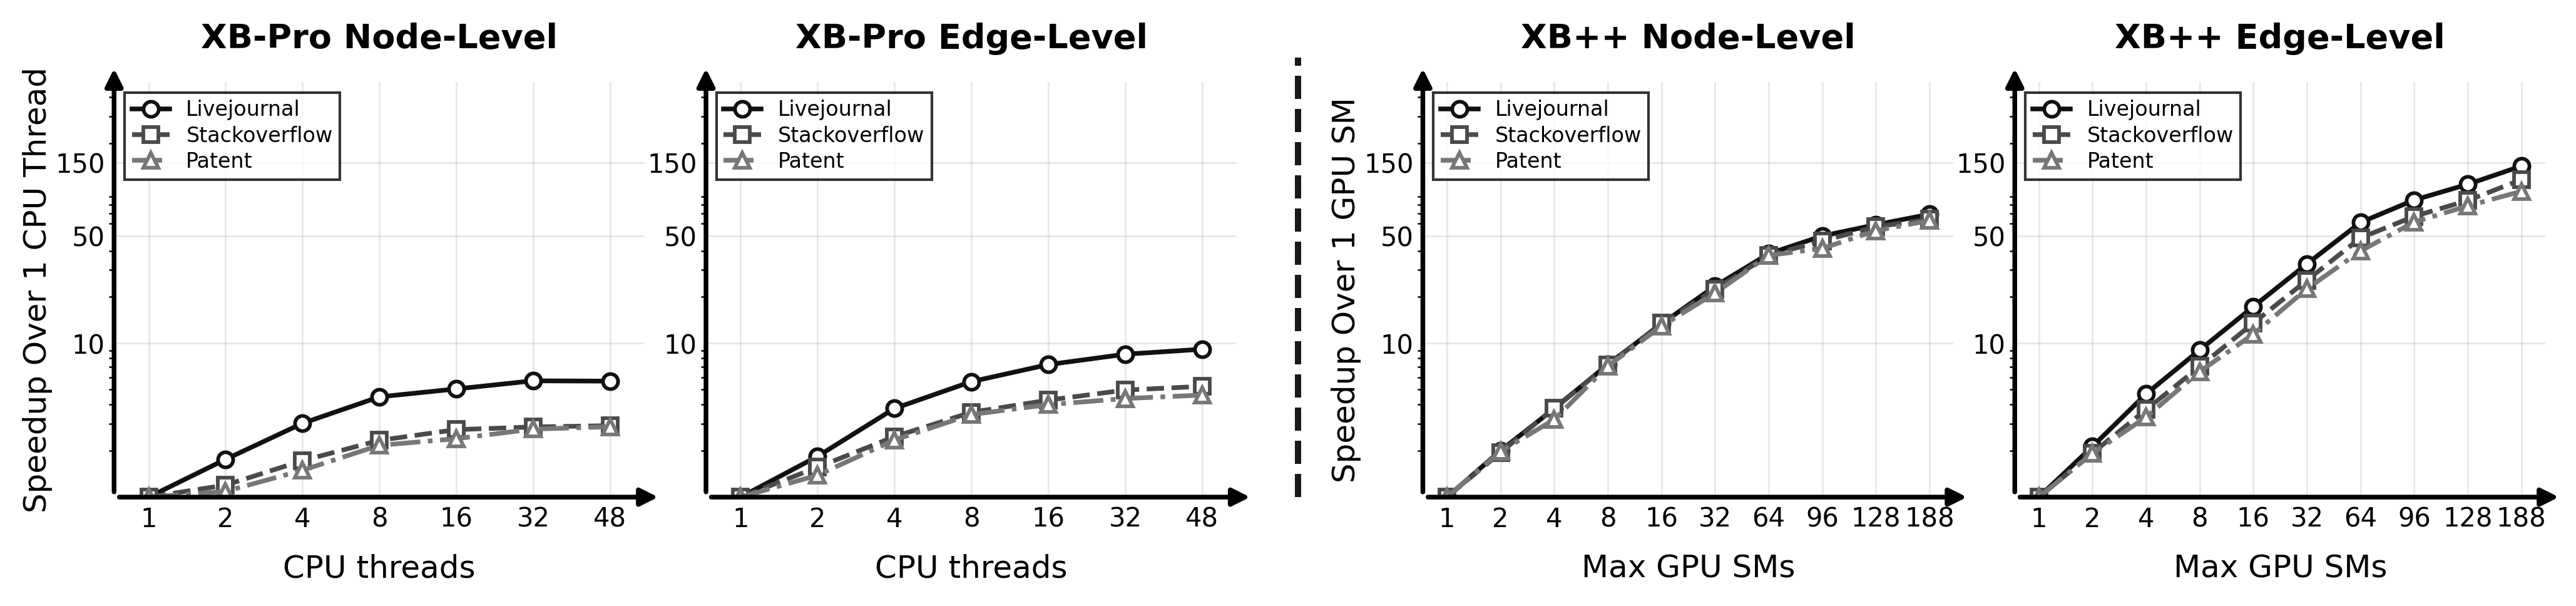
\includegraphics[width=1.0\columnwidth]{figures/plots/plot_scalability.png}
    \captionsetup{skip=4pt}
    \caption{Scalability of XB-Pro and XB++ over one CPU thread or one GPU SM.}
    \label{plot:scalability_test}
\vspace{-4pt}
\end{figure}

\textcolor{blue}{
On both CPU and GPU, edge-level load balancing achieves higher speedups than node-level load balancing on each dataset.
This is because edge-level scheduling exposes finer-grained frontier work, which improves utilization of available execution resources and reduces load imbalance across vertices with different degrees.
The GPU speedups are substantially higher than the CPU speedups as more resources are enabled.
XB++ benefits more from additional GPU SMs because CUDA threads are lightweight and scheduled in warps by hardware, allowing many fine-grained edge tasks to run concurrently and \textcolor{blue}{reduce} amortized memory latency with relatively low scheduling overhead.
In contrast, XB-Pro is limited by the smaller number of CPU cores, heavier software threads, and more expensive synchronization and memory-hierarchy effects, so additional CPU threads provide less aggregate parallel throughput.
}
